\documentclass{article}
\usepackage{fancyhdr} % for pretty formatting
\usepackage{amsmath} % for matrices
\usepackage{amssymb} % for bold text
\usepackage{pgfplots} % for graphs
\usepackage{hyperref} % for hyperlinks
\pgfplotsset{compat=1.18}
\usepackage{enumitem} % for custom lists

\usepackage{lipsum} % For dummy text
\usepackage{cite} % For citations

\pagestyle{fancy}  
\fancyhf{} % Clear all header and footer fields

\usepackage{tcolorbox} % Required for tcolorbox

\newtcolorbox{solutioncheck}{
    colback=green!10, % Background color
    colframe=gray!50, % Frame color
    boxsep=5pt, % Padding
    arc=4pt, % Rounded corners
    title=Checking solution, % Optional title for the aside
    fonttitle=\bfseries, % Title font style
} % for Asides

\lhead{Joshua Dunne}
\rhead{\thepage} % Displays the current page number 
\lfoot{MATH620}
\rfoot{Unit 3}
\cfoot{Homework 4}

\begin{document}
\section{Question 1}
    \paragraph{Given}
        We are given three different vectors to try to map through a
        given function. We are then to plot everything.
        \begin{enumerate}
            \item $\mathbf{A} = \begin{bmatrix}3 & 0\\0 & -2\end{bmatrix}$
            \item $T: \mathbb{R}^2 \rightarrow \mathbb{R}^2 $ 
            \item$T(\mathbf{x})=\mathbf{A}\mathbf{x}$
        \end{enumerate}
    \paragraph{Find}
        \begin{enumerate}
            \item 
                The image of $u$ under $T$ where
                $\mathbf{u} = \begin{bmatrix}3\\-1\end{bmatrix}$
            \item 
                The image of $c$ under $T$ where
                $\mathbf{v} = \begin{bmatrix}0\\1.5\end{bmatrix}$
            \item The image of $\mathbf{u} + \mathbf{v}$
        \end{enumerate}
    \subsection{Work}
        \paragraph{Images}
            The image under is just going to be the result of having the function
            applied. We can do as such like so, for each of the given terms
            \begin{enumerate}
                \item 
                    $T(\mathbf{u}) = A\mathbf{u} = \begin{bmatrix}3 & 0\\0 & -2\end{bmatrix}\begin{bmatrix}3\\-1\end{bmatrix} = \begin{bmatrix}9\\2\end{bmatrix}$
                \item 
                    $T(\mathbf{v}) = A\mathbf{v} = \begin{bmatrix}3 & 0\\0 & -2\end{bmatrix}\begin{bmatrix}0\\1.5\end{bmatrix} = \begin{bmatrix}0\\-3\end{bmatrix}$
                \item 
                    $T(\mathbf{u}+\mathbf{v}) = A(\mathbf{u}+\mathbf{v}) = \begin{bmatrix}3 & 0\\0 & -2\end{bmatrix}\begin{bmatrix}0\\1.5\end{bmatrix} = \begin{bmatrix}9\\-1\end{bmatrix}$
            \end{enumerate}
    \newpage
    \subsection{Illustration}
        \paragraph{Scaling}
            Throughout we should expect to see a few things. The origin
            should remain constant, and relationships about perpendicularity
            and being parallel should contiue to hold.
        \begin{figure}[h!]
            \begin{center}
            \begin{minipage}[b]{0.4\textwidth}
                

            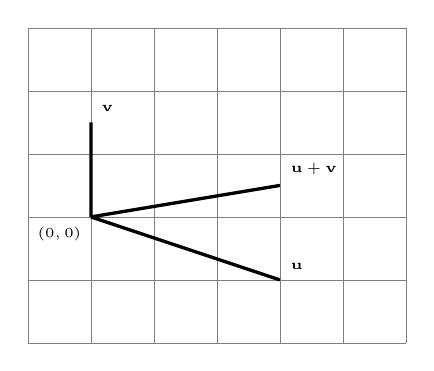
\begin{tikzpicture}[
                    every node/.style={font=\tiny},
                    scale=0.8 % Adjusted scale to fit a reasonable paper size, you can change this
                ]
                
                \draw[step=1.0, gray, very thin] (-1, -2) grid (5, 3);
                \node[below left] at (0,0) {$(0,0)$};
                \draw[very thick]
                    (0, 0) -- (3, -1) node[above right] {$\mathbf{u}$}
                    (0, 0) -- (0, 1.5) node[above right] {$\mathbf{v}$}
                    (0, 0) -- (3, .5) node[above right] {$\mathbf{u} + \mathbf{v}$};
                ;
            \end{tikzpicture}

            
            \end{minipage}
            \hspace{0.5cm}
            \begin{minipage}[b]{0.44\textwidth}
                

            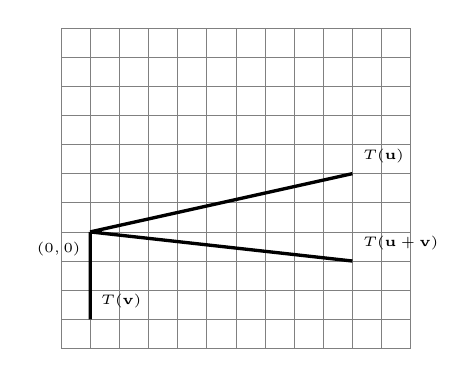
\begin{tikzpicture}[
                    every node/.style={font=\tiny},
                    scale=0.37 % Adjusted scale to fit a reasonable paper size, you can change this
                ]
                
                \draw[step=1.0, gray, very thin] (-1, -4) grid (11, 7);
                \node[below left] at (0,0) {$(0,0)$};
                \draw[very thick]
                    (0, 0) -- (9, 2) node[above right] {$T(\mathbf{u})$}
                    (0, 0) -- (0, -3) node[above right] {$T(\mathbf{v})$}
                    (0, 0) -- (9, -1) node[above right] {$T(\mathbf{u}+\mathbf{v})$};
                ;
            \end{tikzpicture}

             
            \end{minipage} 
            \end{center}
        \end{figure}
    
    \section{Question 2}
        \paragraph{Given}
            the matrix $A$:
            $$
                A = \begin{bmatrix} 1 & -5 & -7 \\ -3 & 7 & 5 \end{bmatrix}
            $$
            Define the linear transformation $T: \mathbb{R}^3 \rightarrow \mathbb{R}^2$ by $T(\mathbf{x}) = A\mathbf{x}$.
        \subsection{Prompts}
            \begin{enumerate}[label=(\alph*)]
                \item 
                    Find the image under T of $\mathbf{u}=\begin{bmatrix}2\\1\\-1\end{bmatrix}$
                    So. We have a 2x3 and we're multiplying by a 3x1. The result is going to be a 2x1
                    \begin{solutioncheck}
                        \[
                        \begin{bmatrix} 1 & -5 & -7 \\ -3 & 7 & 5 \end{bmatrix}
                        \begin{bmatrix}2\\1\\-1\end{bmatrix}
                        =
                        \begin{bmatrix}4\\-4\end{bmatrix}
                        \]
                    \end{solutioncheck}
                \item
                    Find a vector $\mathbf{x}$ whose image under
                    T is $\mathbf{b}=\begin{bmatrix}-12\\12\end{bmatrix}$
                    \paragraph{Thinking}
                        We can se up the system of equations so that we're solving for this.
                        As long as the solution $y\in\text{span}\{\mathbf{u},\mathbf{v}\}$
                    \paragraph{Solution}
                        \[
                        \begin{bmatrix} 1 & -5 & -7 \\ -3 & 7 & 5 \end{bmatrix}
                        \begin{bmatrix}x_1\\x_2\\x_3\end{bmatrix}
                        =
                        \begin{bmatrix}-12\\12\end{bmatrix}
                        \]
                        \begin{align*}
                            x_1 - 5x_2 - 7x_3 &= -12 \\
                            -3x_1 + 7x_2 + 5x_3 &= 12
                        \end{align*}
                        \begin{align*}
                            x_1 + 3x_3 &= 3 \\
                            x_2 + 2x_3 &= 3
                        \end{align*}
                        \subparagraph{Particular solution}
                            Let $x_3=0$ then $x_1=3$ and $x_2=3$.
                        \begin{solutioncheck}
                            \[
                            \begin{bmatrix} 1 & -5 & -7 \\ -3 & 7 & 5 \end{bmatrix}
                            \begin{bmatrix}3\\3\\0\end{bmatrix}
                            =
                            \begin{bmatrix}-12\\12\end{bmatrix}
                            \]
                        \end{solutioncheck}
            \end{enumerate}   

    \section{Question 3}
        \subsection{Restate}
            We're out to show that something is not a linear transformation
        \paragraph{Given}
            \[
                T(\begin{bmatrix}x_1\\x_2\end{bmatrix})
                =
                \begin{bmatrix}x_1+5\\x_2\end{bmatrix}
            \]
        \paragraph{Clarification}
            As was discussed in classes and previously in other classes. The two things
            we need to consider something a linear transformation are
            \begin{itemize}
                \item \textbf{Homogeneity} We need that $T(c\mathbf{v})=cT(\mathbf{v})$,
                $\forall{c}\in\mathbb{R}$
                \item \textbf{Additivity} We need that $T(\mathbf{u}+\mathbf{v})=T(\mathbf{u})+T(\mathbf{v})$
            \end{itemize}
        \subsection{Breaking things}
            Alright. We have two requirements. Let's see which is going
            to be the one to break.
            \paragraph{Additivity}
                
                Let's define two vectors, $\mathbf{u}$ and $\mathbf{v}$, to test this property.
                \[
                    \mathbf{u} = \begin{bmatrix}u_1\\u_2\end{bmatrix}, \quad
                    \mathbf{v} = \begin{bmatrix}v_1\\v_2\end{bmatrix}
                \]
                First, we'll find the sum of the vectors and then apply the transformation $T$.
                \[
                    T(\mathbf{u}+\mathbf{v}) = T\left(\begin{bmatrix}u_1+v_1\\u_2+v_2\end{bmatrix}\right) = \begin{bmatrix}(u_1+v_1)+5\\u_2+v_2\end{bmatrix}
                \]
                Next, we'll apply the transformation to each vector individually and then add the results.
                \[
                    T(\mathbf{u}) = \begin{bmatrix}u_1+5\\u_2\end{bmatrix}, \quad
                    T(\mathbf{v}) = \begin{bmatrix}v_1+5\\v_2\end{bmatrix}
                \]
                \[
                    T(\mathbf{u}) + T(\mathbf{v}) = \begin{bmatrix}u_1+5\\u_2\end{bmatrix} + \begin{bmatrix}v_1+5\\v_2\end{bmatrix} = \begin{bmatrix}u_1+v_1+10\\u_2+v_2\end{bmatrix}
                \]
                By comparing the two outcomes, we can see that $T(\mathbf{u}+\mathbf{v}) \neq T(\mathbf{u}) + T(\mathbf{v})$ because:
                \[
                     \begin{bmatrix}(u_1+v_1)+5\\u_2+v_2\end{bmatrix} \neq \begin{bmatrix}u_1+v_1+10\\u_2+v_2\end{bmatrix}
                \]
                Since the additivity property does not hold, $T$ is not a linear transformation.
                We could go through the trouble to double check the other condition, but,
                there's no need.
    \section{Question 4}
        \subsection{Restated}
            Given $AB$ is defined with $B$ having linearly
            dependent columns. Are the columns of $AB$
            linearly independent? If not, counterexample.
        \subsection{Slow}
            Let's take our time with this one. It doesn't give us as far as
            much to work with as have some of the others previously.
            \paragraph{Given}
                So. The columns of $B$ are linearly dependent.
                We know a few things because of this that are worth listing here before further investigation
                \begin{enumerate}
                    \item We know that we will have a free variable
                    \item That one of the columns can be expressed as a linear combination of the others
                    \item $B\mathbf{x} = \mathbf{0}$ will have a nontrivial solution
                \end{enumerate}
                    From this we can state that there exists a non-zero vector $\mathbf{x}$ such that $B\mathbf{x} = \mathbf{0}$. 
                    This means that at least one column of $B$ can be written as a linear combination of the other columns.
            \paragraph{Deduction}
                \begin{gather*}
                    B\mathbf{x}=\mathbf{0}\text{ for some }\mathbf{x} \\
                    AB\mathbf{x}=(AB)\mathbf{x}=A(B\mathbf{x}) \\
                    A(B\mathbf{x})=A\mathbf{0}=\mathbf{0} 
                \end{gather*}
                So. There exists an $\mathbf{x}$ such that when
                $\mathbf{x}$ is applied to $B$ we get the zero vector. Then, when we apply $A$ to that zero vector, we still get the zero vector.
                This means that $(AB)\mathbf{x} = \mathbf{0}$ has a non-trivial solution (the same $\mathbf{x}$ that makes $B\mathbf{x}=\mathbf{0}$).
                Therefore, the columns of $AB$ are linearly dependent.

            \paragraph{Arr. Thar be a counterexample}
                We could do this backwards as was done above. Find an $\mathbf{x}$
                such that $B\mathbf{x} = \mathbf{0}$. Then we'd easily find a nontrivial
                solution for $AB\mathbf{x}=\mathbf{0}$ 
                \subparagraph{Sounds like alot of work}
                    That sounds like it might take more than a single step, so\dots
                    let's just guess and hope for the best.
                \subparagraph{A guess}
                    Let $A = \begin{bmatrix} 1 & 0 \\ 0 & 1 \end{bmatrix}$ and $B = \begin{bmatrix} 1 & 2 \\ 2 & 4 \end{bmatrix}$.
                    The columns of $B$ are linearly dependent because the second column is twice the first column.
                    Specifically, if $\mathbf{x} = \begin{bmatrix} 2 \\ -1 \end{bmatrix}$, then $B\mathbf{x} = \begin{bmatrix} 1 & 2 \\ 2 & 4 \end{bmatrix} \begin{bmatrix} 2 \\ -1 \end{bmatrix} = \begin{bmatrix} 2-2 \\ 4-4 \end{bmatrix} = \begin{bmatrix} 0 \\ 0 \end{bmatrix}$.
                    Now, let's compute $AB$:
                    \[
                        AB = \begin{bmatrix} 1 & 0 \\ 0 & 1 \end{bmatrix} \begin{bmatrix} 1 & 2 \\ 2 & 4 \end{bmatrix} = \begin{bmatrix} 1 & 2 \\ 2 & 4 \end{bmatrix}
                    \]
                    The columns of $AB$ are $\begin{bmatrix} 1 \\ 2 \end{bmatrix}$ and $\begin{bmatrix} 2 \\ 4 \end{bmatrix}$. These columns are linearly dependent, as the second column is twice the first.
                    And, as expected, $(AB)\mathbf{x} = \begin{bmatrix} 1 & 2 \\ 2 & 4 \end{bmatrix} \begin{bmatrix} 2 \\ -1 \end{bmatrix} = \begin{bmatrix} 0 \\ 0 \end{bmatrix}$, which is a non-trivial solution.
    \section{Question 5}
        We're being asked to tell whether a given transformation
        could have been produced with alinear transformation

        \begin{center}   
        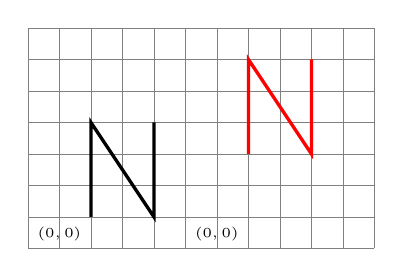
\begin{tikzpicture}[
                every node/.style={font=\tiny},
                scale=0.4 % Adjusted scale to fit a reasonable paper size, you can change this
            ]

            \draw[step=1.0, gray, very thin] (-2, -1) grid (9, 6);

            \node[below left] at (0,0) {$(0,0)$};
            
            \draw[very thick]
                % Bottom-Left E
                (0, 0) -- (0, 3) -- (2, 0) -- (2, 3);
            \draw[very thick, red]
                % Bottom-Left E
                (5, 2) -- (5, 5) -- (7, 2) -- (7, 5);
                
            \node[below left] at (5,0) {$(0,0)$};

        \end{tikzpicture}
        \end{center}
        \subsection{Recent}
            If we look to recent examples we see that this can't work.
            As we saw in the previous problem, 
            a linear transformation must map the zero vector to the zero vector. 
            In this case, the origin $(0,0)$ in the first figure is mapped to $(5,2)$ in the second figure. 
            Since $T(\mathbf{0}) \neq \mathbf{0}$, this transformation cannot be a linear transformation.
    \section{Question 6}
        Lastly, we're going to apply a transformation 
        $C=\begin{bmatrix}2&0\\0&-1.5\end{bmatrix}$
        to\dots a diagram consisting of 10 points this time.
        \paragraph{Aggregating}
            Let's build a long rowed vector like for Unit 3 Task 2.
            \[
                \begin{bmatrix}2&0\\0&-1.5\end{bmatrix}
                \begin{bmatrix}
                    -2&2&2&-2&-1&1&-1&1&-1&1 \\
                    2&2&-2&-2&1&1&-1&-1&-1.5&-1.5
                \end{bmatrix}
            \]
            So, a 2x2 matrix and a 2x10. We get a 2x10 matrix.
            \[
                \begin{bmatrix}
                    -4&4&4&-4&-2&2&-2&2&-2&2 \\
                    -3&-3&3&3&-1.5&-1.5&1.5&1.5&2.25&2.25
                \end{bmatrix}
            \]
            Where we'd take ordered pairs of form
            \[
                (a_{1,0}, a_{2,0}), (a_{1,1}, a_{2,1}), \dots, (a_{1,9}, a_{2,9})
            \]
        \subsection{Plotting a plotting}
                With all this we can reuse some old latex and slap things in a graph
                \begin{center}   
            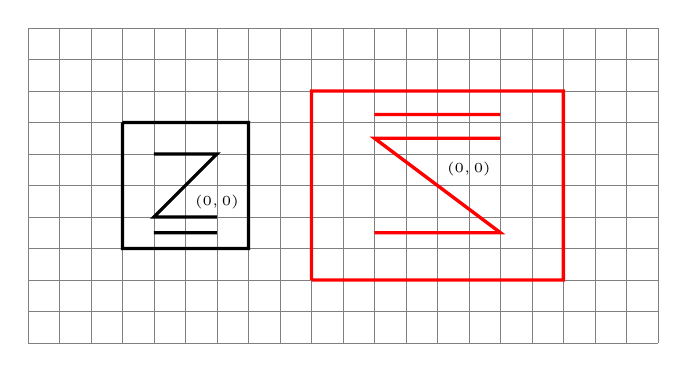
\begin{tikzpicture}[
                every node/.style={font=\tiny},
                scale=0.4% Adjusted scale to fit a reasonable paper size, you can change this
            ]

                \draw[step=1.0, gray, very thin] (-5, -5) grid (15, 5);

                \node[below right] at (0,0) {$(0,0)$};
                
                \draw[very thick]
                    (-2,2)--(2,2)--(2,-2)--(-2,-2)--(-2,2)
                    (-1,1)--(1,1)--(-1,-1)--(1,-1)
                    (-1,-1.5)--(1,-1.5);

                \node[above right] at (8,0) {$(0,0)$};


                \draw[very thick, red]
                    (4,-3)--(12,-3)--(12,3)--(4,3)--(4,-3)
                    (6,-1.5)--(10,-1.5)--(6,1.5)--(10,1.5)
                    (6,2.25)--(10,2.25);

            \end{tikzpicture}
            \end{center}
\end{document}